
%(BEGIN_QUESTION)
% Copyright 2010, Tony R. Kuphaldt, released under the Creative Commons Attribution License (v 1.0)
% This means you may do almost anything with this work of mine, so long as you give me proper credit

Determine the value of the specified {\it integral} for this function:

$$\includegraphics[width=15.5cm]{i04384x01.eps}$$

$$\int_{-5}^{+4} f(x) \> dx$$

\vskip 20pt \vbox{\hrule \hbox{\strut \vrule{} {\bf Suggestions for Socratic discussion} \vrule} \hrule}

\begin{itemize}
\item{} A helpful hint when evaluating integrals is to determine the {\it sign} of the terms within the integrand over the specified interval.  Here, where the interval begins at $x=-5$ and continues to $x=+4$, what is the mathematical sign of $dt$?  Over this same interval, what is the mathematical sign of $f(x)$?
\item{} What is most important when solving problems such as this is to be able to explain {\it why} (not just {\it how}) to arrive at the correct value.  Try explaining the process of integration in your own words, as it applies to this particular problem.
\end{itemize}

\underbar{file i04384}
%(END_QUESTION)





%(BEGIN_ANSWER)

0

%(END_ANSWER)





%(BEGIN_NOTES)


%INDEX% Mathematics, calculus: integral (approximating integral values between points on graph)

%(END_NOTES)


